\documentclass{article}

\usepackage{Sweave}
\begin{document}
\Sconcordance{concordance:seguimientov4.tex:seguimientov4.Rnw:%
1 2 1 1 0 16 1 1 6 1 17 31 0 1 2 2 1 1 9 18 0 1 2 1 1 1 4 5 0 1 3 4 0 1 %
6 4 0 1 3 4 0 1 10 1 0 1 4 2 1 1 9 12 0 1 2 1 1 1 4 5 0 1 3 4 0 1 6 4 0 %
1 3 4 0 1 10 1 0 1 4 2 1 1 9 7 0 1 2 1 1 1 4 5 0 1 3 4 0 1 6 4 0 1 3 4 %
0 1 10 1 0 1 4 3 1 1 9 7 0 1 2 1 1 1 4 5 0 1 3 4 0 1 6 4 0 1 3 4 0 1 10 %
1 0 1 4 3 1 1 9 7 0 1 2 1 1 1 4 5 0 1 3 4 0 1 6 4 0 1 3 4 0 1 10 1 0 1 %
4 3 1 1 9 7 0 1 2 1 1 1 4 5 0 1 3 4 0 1 6 4 0 1 3 4 0 1 10 1 0 1 4 2 1 %
1 9 7 0 1 2 1 1 1 4 5 0 1 3 4 0 1 6 4 0 1 3 4 0 1 10 1 0 1 4 3 1 1 9 7 %
0 1 2 1 1 1 4 5 0 1 3 4 0 1 6 4 0 1 3 4 0 1 10 1 0 1 4 3 1}

\title{PROMSACE: Seguimiento de encuestas}
\author{Hernan Nuñez}
\date{\today}
\maketitle
\begin{abstract}
Lo mostrado en este documento nos da una vision descriptiva y exploratoria sobre los cambios a traves del tiempo (del 28 febrero al 22 de julio) de las encuestas recopiladas y completas. Se trabajo con Latex y RStudio. Pueden encontrar el codigo en https://github.com/HernanPerci/PROMSACE
\end{abstract}

\tableofcontents

\section{Introduccion}
La encuesta sobre la que se respalda el presente informe aun se esta recolectando mediante la platafoma surveymonkey.

\section{Variables de estudio}


\begin{Schunk}
\begin{Soutput}
Rows: 2,258
Columns: 26
$ Fecha                                                                 <dttm> ...
$ `Traba administrativa`                                                <chr> ...
$ `Recursos humanos`                                                    <chr> ...
$ Abastecimiento                                                        <chr> ...
$ `Presupuesto público`                                                 <chr> ...
$ Tesorería                                                             <chr> ...
$ Contabilidad                                                          <chr> ...
$ `Control (previo, simultáneo, concurrente, auditorías externas etc.)` <chr> ...
$ `Inversión pública`                                                   <chr> ...
$ `Planeamiento estratégico`                                            <chr> ...
$ `Modernización de la Gestión Pública`                                 <chr> ...
$ `No sé`                                                               <chr> ...
$ Otro                                                                  <chr> ...
$ `Cambiar el marco normativo`                                          <chr> ...
$ `Potenciar conocimientos y habilidades de los servidores civiles`     <chr> ...
$ `Articular labores entre áreas`                                       <chr> ...
$ `Mejorar los sistemas informáticos y sistematizar procesos`           <chr> ...
$ `Mejorar la coordinación con el ente rector y otras instituciones`    <chr> ...
$ `Entidad publica`                                                     <chr> ...
$ Identificado                                                          <chr> ...
$ Priorizado                                                            <chr> ...
$ `Nivel de gobierno`                                                   <chr> ...
$ `Organo de pertenencia`                                               <fct> ...
$ Sexo                                                                  <chr> ...
$ `Años trabajando en el Estado`                                        <chr> ...
$ completa                                                              <chr> ...
\end{Soutput}
\end{Schunk}

\section{Analisis de la Pregunta 2: Ayúdanos a entender mejor el problema ¿Sabes con qué sistema administrativo se relaciona la experiencia relatada? Si lo sabes, marca hasta dos opciones.}

\begin{Schunk}
\begin{Soutput}
Rows: 2,108
Columns: 13
$ Fecha                                                                 <dttm> ...
$ `Recursos humanos`                                                    <chr> ...
$ Abastecimiento                                                        <chr> ...
$ `Presupuesto público`                                                 <chr> ...
$ Tesorería                                                             <chr> ...
$ Contabilidad                                                          <chr> ...
$ `Control (previo, simultáneo, concurrente, auditorías externas etc.)` <chr> ...
$ `Inversión pública`                                                   <chr> ...
$ `Planeamiento estratégico`                                            <chr> ...
$ `Modernización de la Gestión Pública`                                 <chr> ...
$ `No sé`                                                               <chr> ...
$ Otro                                                                  <chr> ...
$ `Nivel de gobierno`                                                   <chr> ...
\end{Soutput}
\end{Schunk}


\begin{Schunk}
\begin{Soutput}
.
   2    3    4    5    6    7 
 157 1713   74   97   46   21 
\end{Soutput}
\begin{Soutput}
.
 Ene  Feb  Mar  Abr  May  Jun  Jul  Ago  Set  Oct  Nov  Dic 
   0  157 1713   74   97   46   21    0    0    0    0    0 
\end{Soutput}
\begin{Soutput}
.
  1   2   3   4   5   6   7 
 59 454 414 395 334 385  67 
\end{Soutput}
\begin{Soutput}
.
dom lun mar mié jue vie sáb 
 59 454 414 395 334 385  67 
\end{Soutput}
\end{Schunk}
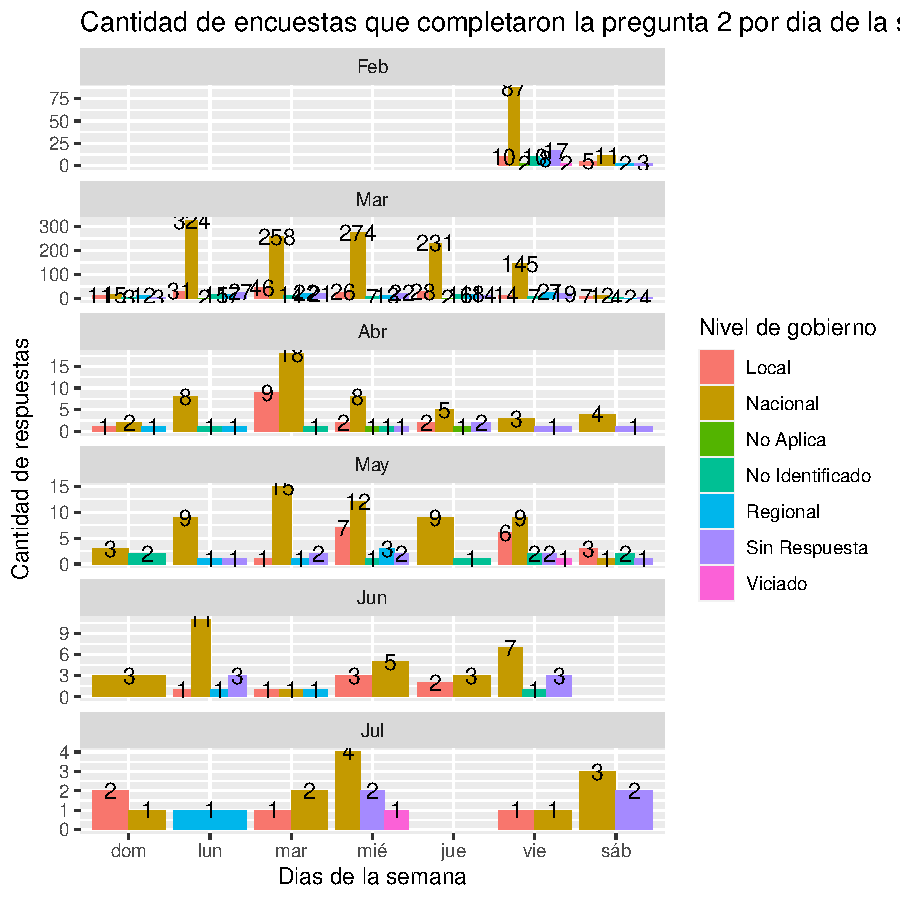
\includegraphics{seguimientov4-004}

\section{Analisis de la pregunta 3: ¿Cuáles de las siguientes acciones crees que deberíamos realizar para solucionar el problema que nos comentaste? Marca hasta dos opciones.}

\begin{Schunk}
\begin{Soutput}
Rows: 2,066
Columns: 7
$ Fecha                                                              <dttm> ...
$ `Cambiar el marco normativo`                                       <chr> ...
$ `Potenciar conocimientos y habilidades de los servidores civiles`  <chr> ...
$ `Articular labores entre áreas`                                    <chr> ...
$ `Mejorar los sistemas informáticos y sistematizar procesos`        <chr> ...
$ `Mejorar la coordinación con el ente rector y otras instituciones` <chr> ...
$ `Nivel de gobierno`                                                <chr> ...
\end{Soutput}
\end{Schunk}


\begin{Schunk}
\begin{Soutput}
.
   2    3    4    5    6    7 
 151 1683   74   95   44   19 
\end{Soutput}
\begin{Soutput}
.
 Ene  Feb  Mar  Abr  May  Jun  Jul  Ago  Set  Oct  Nov  Dic 
   0  151 1683   74   95   44   19    0    0    0    0    0 
\end{Soutput}
\begin{Soutput}
.
  1   2   3   4   5   6   7 
 59 446 409 385 329 376  62 
\end{Soutput}
\begin{Soutput}
.
dom lun mar mié jue vie sáb 
 59 446 409 385 329 376  62 
\end{Soutput}
\end{Schunk}
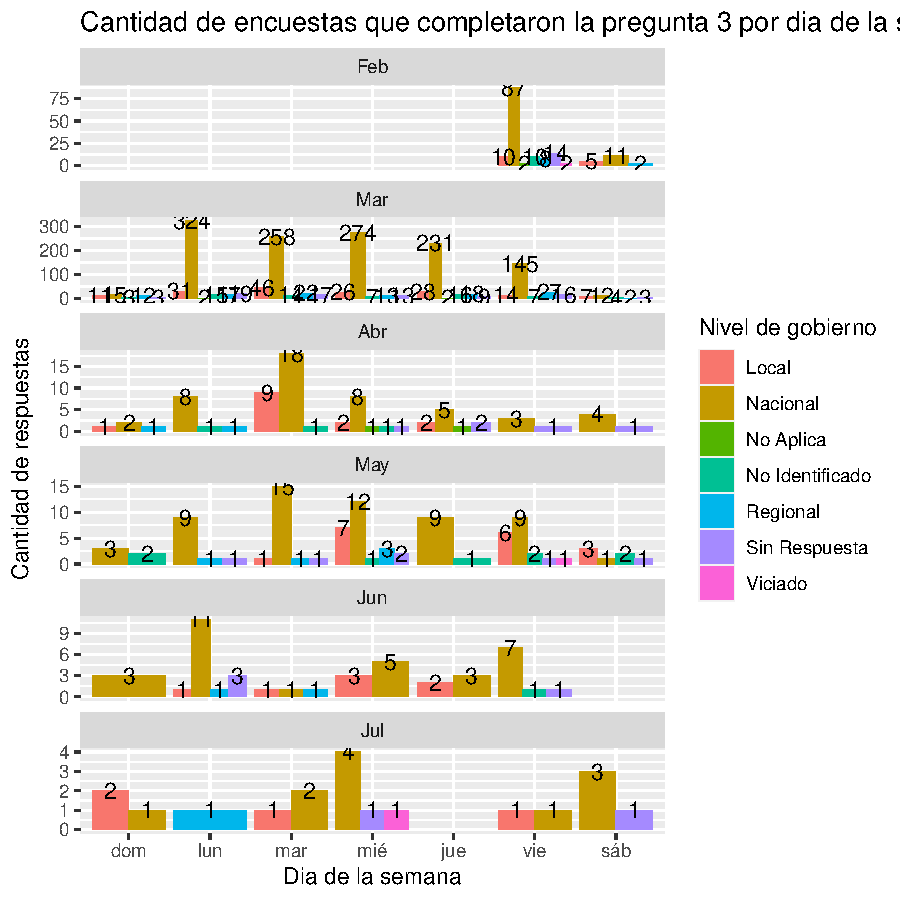
\includegraphics{seguimientov4-006}

\section{Encuestas identificadas}

\begin{Schunk}
\begin{Soutput}
Rows: 1,955
Columns: 2
$ Fecha        <dttm> 2020-07-22 10:17:26, 2020-07-21 17:50:39, 2020-07-21 ...
$ Identificado <chr> "Identificado", "Identificado", "Identificado", "Ident...
\end{Soutput}
\end{Schunk}


\begin{Schunk}
\begin{Soutput}
.
   2    3    4    5    6    7 
 137 1603   69   89   40   17 
\end{Soutput}
\begin{Soutput}
.
 Ene  Feb  Mar  Abr  May  Jun  Jul  Ago  Set  Oct  Nov  Dic 
   0  137 1603   69   89   40   17    0    0    0    0    0 
\end{Soutput}
\begin{Soutput}
.
  1   2   3   4   5   6   7 
 56 423 391 368 318 343  56 
\end{Soutput}
\begin{Soutput}
.
dom lun mar mié jue vie sáb 
 56 423 391 368 318 343  56 
\end{Soutput}
\end{Schunk}
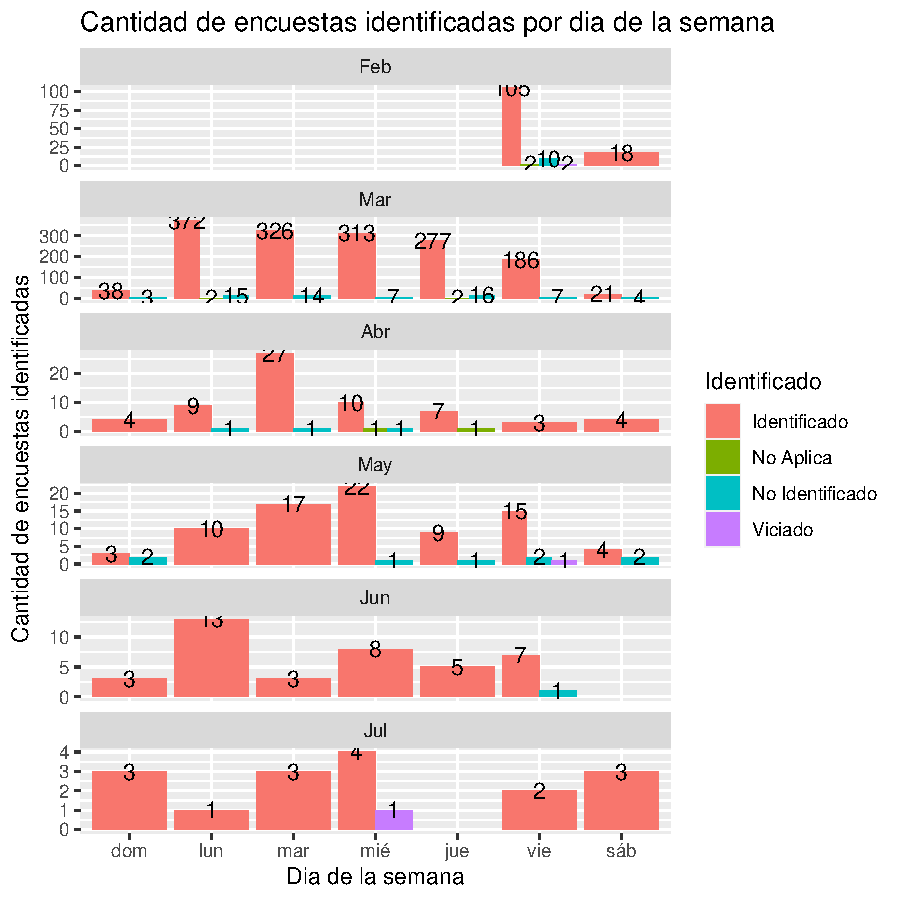
\includegraphics{seguimientov4-008}


\section{Encuestas priorizadas}

\begin{Schunk}
\begin{Soutput}
Rows: 1,955
Columns: 2
$ Fecha      <dttm> 2020-07-22 10:17:26, 2020-07-21 17:50:39, 2020-07-21 11...
$ Priorizado <chr> "Si", "Si", "Si", "Si", "No", "Si", "Viciado", "Si", "Si...
\end{Soutput}
\end{Schunk}


\begin{Schunk}
\begin{Soutput}
.
   2    3    4    5    6    7 
 137 1603   69   89   40   17 
\end{Soutput}
\begin{Soutput}
.
 Ene  Feb  Mar  Abr  May  Jun  Jul  Ago  Set  Oct  Nov  Dic 
   0  137 1603   69   89   40   17    0    0    0    0    0 
\end{Soutput}
\begin{Soutput}
.
  1   2   3   4   5   6   7 
 56 423 391 368 318 343  56 
\end{Soutput}
\begin{Soutput}
.
dom lun mar mié jue vie sáb 
 56 423 391 368 318 343  56 
\end{Soutput}
\end{Schunk}
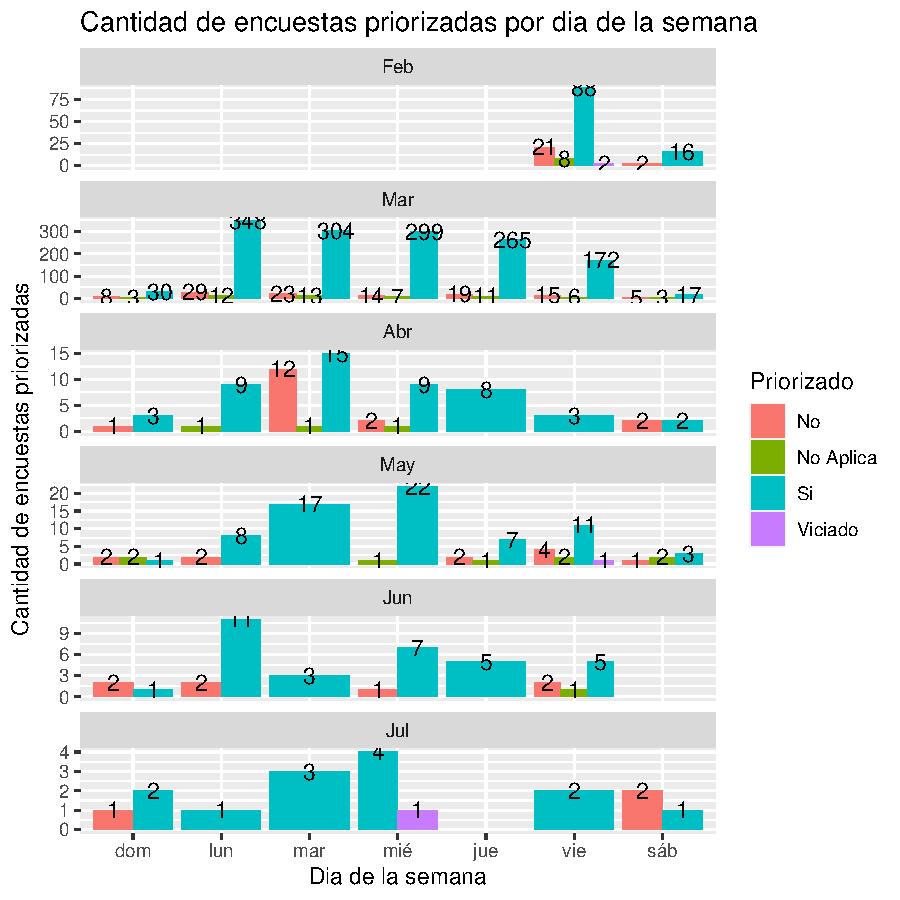
\includegraphics{seguimientov4-010}


\section{Nivel de gobierno}

\begin{Schunk}
\begin{Soutput}
Rows: 1,955
Columns: 2
$ Fecha               <dttm> 2020-07-22 10:17:26, 2020-07-21 17:50:39, 2020...
$ `Nivel de gobierno` <chr> "Nacional", "Nacional", "Local", "Nacional", "N...
\end{Soutput}
\end{Schunk}


\begin{Schunk}
\begin{Soutput}
.
   2    3    4    5    6    7 
 137 1603   69   89   40   17 
\end{Soutput}
\begin{Soutput}
.
 Ene  Feb  Mar  Abr  May  Jun  Jul  Ago  Set  Oct  Nov  Dic 
   0  137 1603   69   89   40   17    0    0    0    0    0 
\end{Soutput}
\begin{Soutput}
.
  1   2   3   4   5   6   7 
 56 423 391 368 318 343  56 
\end{Soutput}
\begin{Soutput}
.
dom lun mar mié jue vie sáb 
 56 423 391 368 318 343  56 
\end{Soutput}
\end{Schunk}
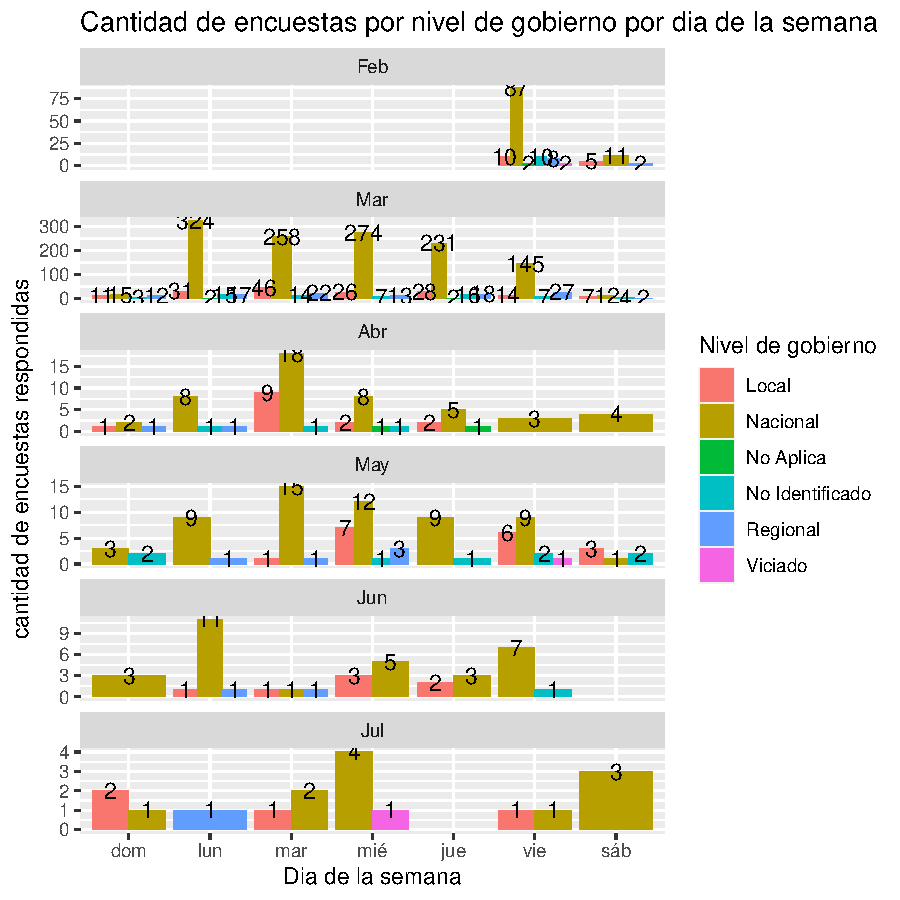
\includegraphics{seguimientov4-012}


\section{Organo de pertenencia}

\begin{Schunk}
\begin{Soutput}
Rows: 1,955
Columns: 2
$ Fecha                   <dttm> 2020-07-22 10:17:26, 2020-07-21 17:50:39, ...
$ `Organo de pertenencia` <fct> linea, apoyo, asesoria, linea, apoyo, apoyo...
\end{Soutput}
\end{Schunk}


\begin{Schunk}
\begin{Soutput}
.
   2    3    4    5    6    7 
 137 1603   69   89   40   17 
\end{Soutput}
\begin{Soutput}
.
 Ene  Feb  Mar  Abr  May  Jun  Jul  Ago  Set  Oct  Nov  Dic 
   0  137 1603   69   89   40   17    0    0    0    0    0 
\end{Soutput}
\begin{Soutput}
.
  1   2   3   4   5   6   7 
 56 423 391 368 318 343  56 
\end{Soutput}
\begin{Soutput}
.
dom lun mar mié jue vie sáb 
 56 423 391 368 318 343  56 
\end{Soutput}
\end{Schunk}
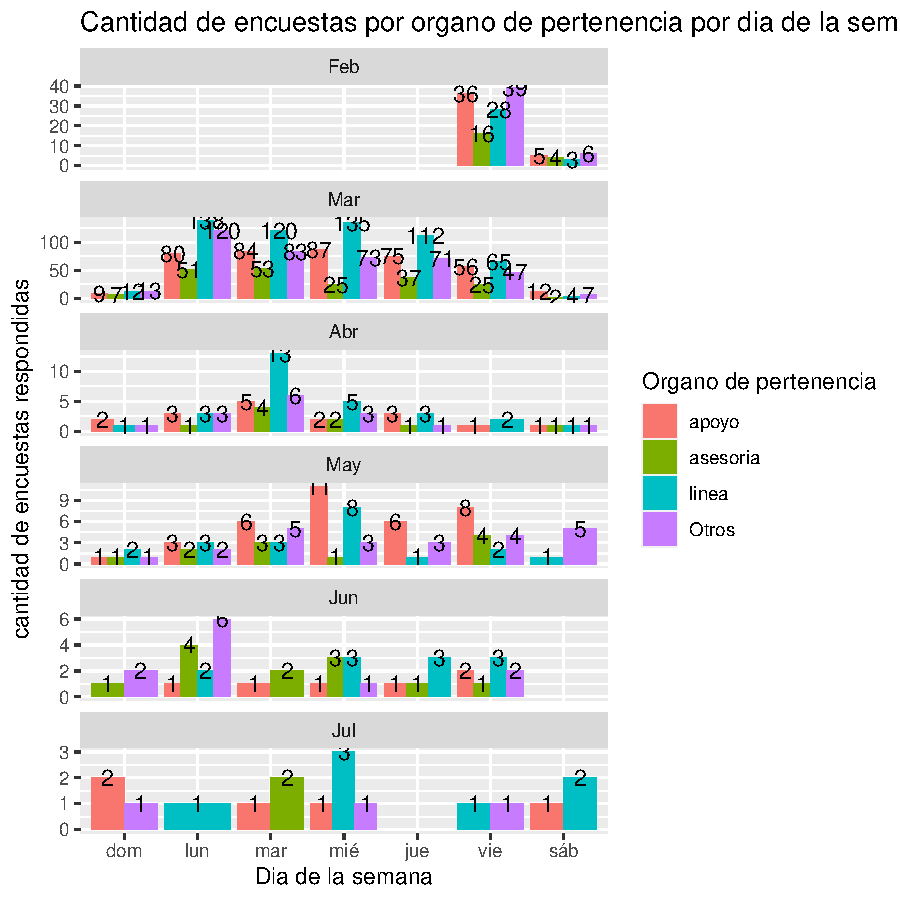
\includegraphics{seguimientov4-014}

\section{Sexo}

\begin{Schunk}
\begin{Soutput}
Rows: 1,955
Columns: 2
$ Fecha <dttm> 2020-07-22 10:17:26, 2020-07-21 17:50:39, 2020-07-21 11:39:2...
$ Sexo  <chr> "Mujer", "Hombre", "Hombre", "Hombre", "Hombre", "Hombre", "H...
\end{Soutput}
\end{Schunk}


\begin{Schunk}
\begin{Soutput}
.
   2    3    4    5    6    7 
 137 1603   69   89   40   17 
\end{Soutput}
\begin{Soutput}
.
 Ene  Feb  Mar  Abr  May  Jun  Jul  Ago  Set  Oct  Nov  Dic 
   0  137 1603   69   89   40   17    0    0    0    0    0 
\end{Soutput}
\begin{Soutput}
.
  1   2   3   4   5   6   7 
 56 423 391 368 318 343  56 
\end{Soutput}
\begin{Soutput}
.
dom lun mar mié jue vie sáb 
 56 423 391 368 318 343  56 
\end{Soutput}
\end{Schunk}
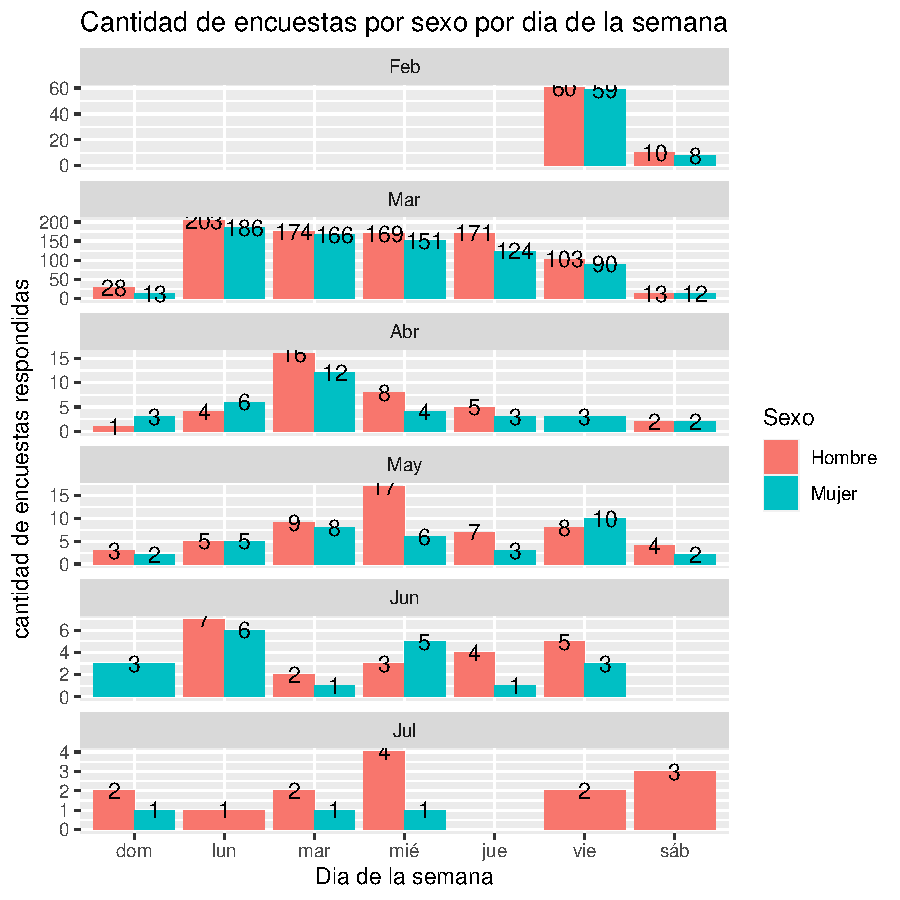
\includegraphics{seguimientov4-016}


\section{Años trabajando en el estado}

\begin{Schunk}
\begin{Soutput}
Rows: 1,955
Columns: 2
$ Fecha                          <dttm> 2020-07-22 10:17:26, 2020-07-21 17:...
$ `Años trabajando en el Estado` <chr> "De seis a diez años", "De seis a di...
\end{Soutput}
\end{Schunk}


\begin{Schunk}
\begin{Soutput}
.
   2    3    4    5    6    7 
 137 1603   69   89   40   17 
\end{Soutput}
\begin{Soutput}
.
 Ene  Feb  Mar  Abr  May  Jun  Jul  Ago  Set  Oct  Nov  Dic 
   0  137 1603   69   89   40   17    0    0    0    0    0 
\end{Soutput}
\begin{Soutput}
.
  1   2   3   4   5   6   7 
 56 423 391 368 318 343  56 
\end{Soutput}
\begin{Soutput}
.
dom lun mar mié jue vie sáb 
 56 423 391 368 318 343  56 
\end{Soutput}
\end{Schunk}
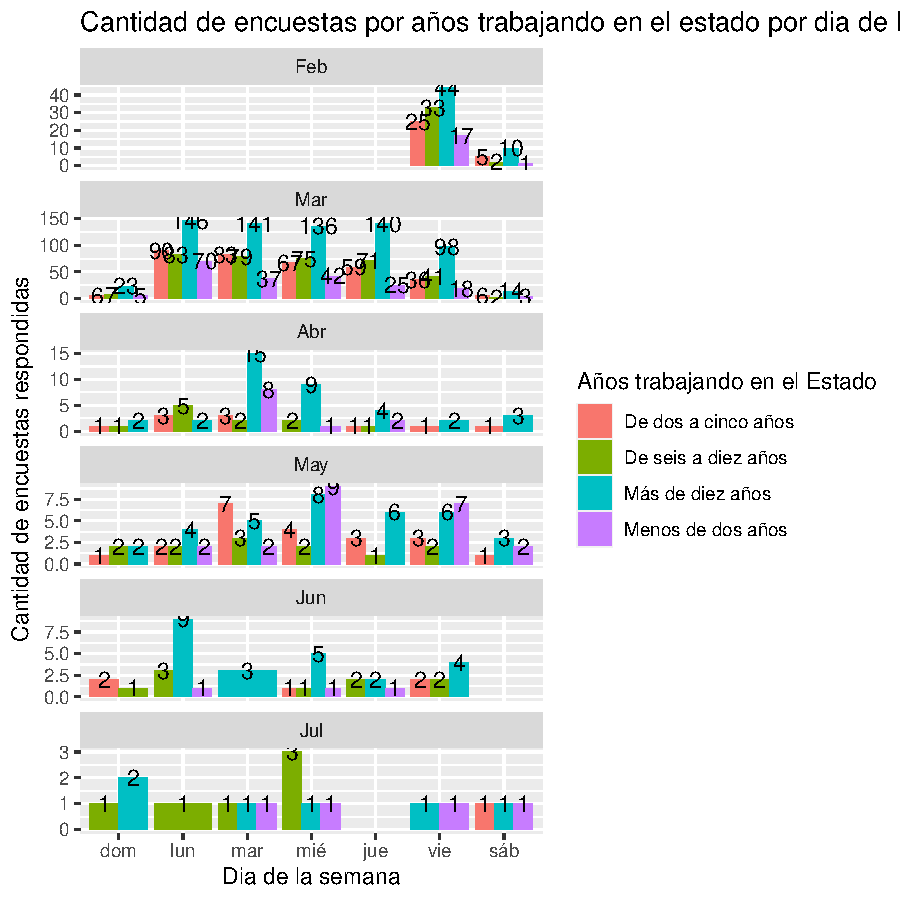
\includegraphics{seguimientov4-018}



\end{document}
